\section{Applications of Double Integrals} \label{S:11.4.Double_Integrals_Applications}

\vspace*{-14 pt}
\framebox{\hspace*{3 pt}
\parbox{6.25 in}{\begin{goals}
\item If we have a mass density function for a lamina (thin plate), how does a double integral determine the mass of the lamina?

\item How may a double integral be used to find the area between two curves?

\item Given a mass density function on a lamina, how can we find the lamina's center of mass?
\item What is a joint probability density function? How do we determine the probability of an event if we know a probability density function?
\end{goals}} \hspace*{3 pt}}

\subsection*{Introduction}

So far, we have interpreted the double integral of a function $f$ over a domain $D$ in two different ways. First, $\iint_D f(x,y) \, dA$ tells us a difference of volumes -- the volume the surface defined by $f$ bounds above the $xy$-plane on $D$ minus the volume the surface bounds below the $xy$-plane on $D$.  In addition, $\frac{1}{A(D)} \iint_D f(x,y) \, dA$ determines the average value of $f$ on $D$. In this section, we investigate several other applications of double integrals, using the integration process as seen in Preview Activity \ref{PA:11.4}: we partition into small regions, approximate the  desired quantity on each small region, then use the integral to sum these values exactly in the limit.

The following preview activity explores how a double integral can be used to determine the density of a thin plate with a mass density distribution.  Recall that in single-variable calculus, we considered a similar problem and computed the mass of a one-dimensional rod with a mass-density distribution.  There, as here, the key idea is that if density is constant, mass is the product of density and volume.

\begin{pa} \label{PA:11.4} Suppose that we have a flat, thin object (called a \emph{lamina}) whose density varies across the object. We can think of the density on a lamina as a measure of mass per unit area. As an example, consider a circular plate $D$ of radius 1 cm centered at the origin whose density $\delta$ varies depending on the distance from its center so that  the density in grams per square centimeter at point $(x, y)$ is
\[\delta(x,y) = 10-2(x^2+y^2).\]

    \ba
    \item %Assume the density is 0 at any point outside of the disk.  
    Suppose that we partition the plate into subrectangles $R_{ij}$, where $1 \leq i \leq m$ and $1 \leq j \leq n$, of equal area $\Delta A$, and select a point $(x_{ij}^*,y_{ij}^*)$ in $R_{ij}$ for each $i$ and $j$.
    
    What is the meaning of the quantity $\delta(x_{ij}^*,y_{ij}^*) \Delta A$?
    
%        \begin{enumerate}[i.]
 %       \item Find a reasonable approximation of the mass of the plate on the subrectangle $R_{ij}$. Explain why you have a reasonable approximation. (Hint: mass is density times area if density is constant.)

        \item State a double Riemann sum that provides an approximation of the mass of the plate.


        \item Explain why the double integral
    \[\iint_D \delta(x,y) \, dA\]
    tells us the exact mass of the plate.


        \item Determine an iterated integral which, if evaluated, would give the exact mass of the plate.  Do not actually evaluate the integral.\footnote{This integral is considerably easier to evaluate in polar coordinates, which we will learn more about in Section~\ref{S:11.5.Double_Integrals_Polar}.}


    %\end{enumerate}
\ea

\end{pa}

\begin{activitySolution} 

    \ba
    \item If we assume the density is the constant $\delta(x_{ij}^*,y_{ij}^*)$ on $R_{ij}$, then the quantity
\[\delta(x_{ij}^*,y_{ij}^*) \Delta A\]
is a density times area and $\delta(x_{ij}^*,y_{ij}^*) \Delta A$ approximates the mass of the chunk of the plate over $R_{ij}$.

        \item To approximate the mass of the plate, we add the approximations on each subrectangle to obtain
\[\sum_{i=1}^m \sum_{j=1}^n \delta(x_{ij}^*,y_{ij}^*) \Delta A,\]
which approximates the total mass of the plate.


        \item If we take the limit of the sum in part (b) as the number of subrectangles goes to infinity, we are adding masses over smaller and smaller subrectangles, so in the limit 
\[\lim_{\Delta A \to 0} \sum_{i=1}^m \sum_{j=1}^n \delta(x_{ij}^*,y_{ij}^*) \Delta A = \iint_D \delta(x,y) \, dA,\]
the double integral gives the total mass of the plate.

        \item The mass of our plate in this example is
\[\iint_D \delta(x,y) \, dA = \iint_D 10-2(x^2+y^2) \, dA.\]
%This integral is probably easier to integrate in polar coordinates. The density $\delta$ is represented in polar coordinates as
%\[\delta(r,\theta) = 10 - 2r^2\]
%and the domain $D$ is described by
%\[0 \leq r \leq 1 \ \ \ \ \ \text{ and } \ \ \ \ \ 0 \leq \theta \leq 2\pi.\]
%Therefore, the mass of the plate is
%\begin{align*}
%\iint_D 10-2(x^2+y^2) \, dA &= \int_{0}^{2\pi} \int_{0}^{1} \delta(r,\theta) \, r \, dr \, d\theta \\
%	&= \int_{0}^{2\pi} \int_{0}^{1} 10r - 2r^3 \, dr \, d\theta \\
%	&= \int_{0}^{2\pi} \left[5r^2 - \frac{1}{4}r^4\right]\biggm|_{0}^{1} \, d\theta \\
%	&= \int_{0}^{2\pi} \frac{9}{2} \, d\theta \\
%	&= \frac{9}{2}\theta \bigm|_0^{2\pi}  \\
%	&= 9 \pi.
%\end{align*}


\ea
\end{activitySolution}
 \afterpa 

\subsection*{Mass}

Density is a measure of some quantity per unit area or volume. For example, we can measure the human population density of some region as the number of humans in that region divided by the area of that region. In physics, the mass density of an object is the mass of the object per unit area or volume.  As suggested by Preview Activity~\ref{PA:11.4}, the following holds in general.

 \vspace*{5pt}
\nin \framebox{\hspace*{3 pt}
\parbox{6.25 in}{If $\delta(x, y)$ describes the density of a lamina defined by a planar region $D$, then the \textbf{mass}\index{double integral!mass of lamina} of $D$ is given by the double integral $\ds \iint_D \delta(x,y) \, dA$.
} \hspace*{3 pt}}
\vspace*{5pt}

\begin{activity} \label{A:11.4.3} Let $D$ be a half-disk lamina of radius 3 in quadrants IV and I, centered at the origin as shown in Figure \ref{F:11.4.Mass_exercise}. Assume the density at point $(x,y)$ is given by $\delta(x,y) = x$. Find the exact mass of the lamina.

\begin{figure}[ht]
\begin{center}
%\resizebox{!}{2.4in}{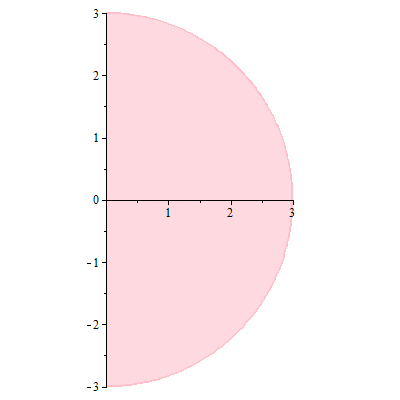
\includegraphics{11_4_Mass_exercise}}
  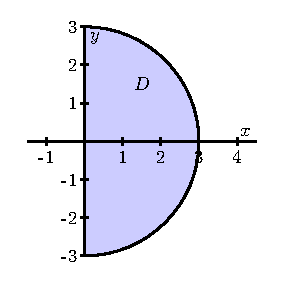
\includegraphics{figures/fig_11_4_half_circle.eps}
\end{center}
\caption{A half disk lamina.}
\label{F:11.4.Mass_exercise}
\end{figure}

\end{activity}
\begin{smallhint}

\end{smallhint}
\begin{bighint}

\end{bighint}
\begin{activitySolution}
We integrate the density over the region $D$. We have $\delta(x,y) = x$, and the region $D$ can be described by $0 \leq x \leq \sqrt{9-y^2}$ for $y$ between $-3$ and $3$. Thus, the mass of the lamina is
\begin{align*}
\int_{-3}^{3} \int_{0}^{\sqrt{9-y^2}} x \, dx \, dy &= \int_{-3}^{3} \left. \frac{x^2}{2} \right|_{0}^{\sqrt{9-y^2}} \, dy \\
	&= \int_{-3}^{3} \frac{1}{2}(9-y^2) \, dy \\
	&= \frac{1}{2} \left. \left[9y - \frac{1}{3}y^3\right]\right|_{-3}^{3} \\
	&= 18.
\end{align*}
\end{activitySolution}
\aftera


\subsection*{Area}

If we consider the situation where the mass-density distribution is constant, we can also see how a double integral may be used to determine the area of a region.  Assuming that $\delta(x,y) = 1$ over a closed bounded region $D$, where the units of $\delta$ are ``mass per unit of area,'' it follows that $\iint_D 1 \, dA$ is the mass of the lamina.  But since the density is constant, the numerical value of the integral is simply the area. 

As the following activity demonstrates, we can also see this fact by considering a three-dimensional solid whose height is always 1.  %We have used a single integral to calculate the areas of regions in the plane. The double integral can be used to calculate areas\index{double integral!area between curves} as well.

\begin{activity} \label{A:11.4.1} Suppose we want to find the area of the bounded region $D$ between the curves
\[y = 1-x^2 \ \ \ \ \ \text{ and } \ \ \ \ \ y=x-1.\]
A picture of this region is shown in Figure \ref{F:11.4.Area_ex_1}. 

\ba
	\item We know that the volume of a solid with constant height is given by the area of the base times the height.  Hence, we may interpret the area of the region $D$ as the volume of a solid with base $D$ and of uniform height 1.  Determine a double integral whose value is the area of $D$. 
\begin{figure}[ht]
\begin{center}
%\resizebox{!}{2.4in}{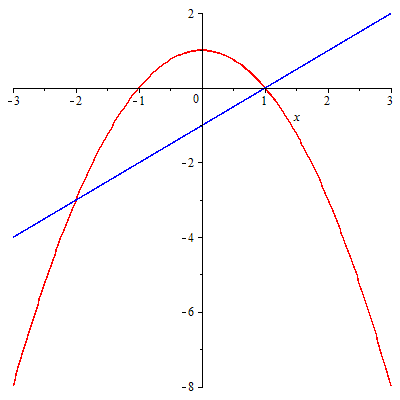
\includegraphics{11_4_Area_ex_1}}
  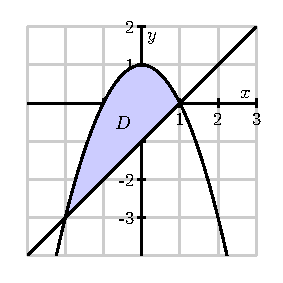
\includegraphics{figures/fig_11_4_area.eps}
\end{center}
\caption{The graphs of $y = 1-x^2$ and $y=x-1$.}
\label{F:11.4.Area_ex_1}
\end{figure}

	\item Write an iterated integral whose value equals the double integral you found in (a).
	\item Use the Fundamental Theorem of Calculus to evaluate \emph{only} the inner integral in the iterated integral in (b).  
	\item After completing part (c), you should see a standard single area integral from calc II. Evaluate this remaining integral to find the exact area of $D$.
\ea

\end{activity}
\begin{smallhint}

\end{smallhint}
\begin{bighint}

\end{bighint}
\begin{activitySolution}
\ba
\item The double integral
\[\int \int_D 1 \, dA\]
gives the volume of the solid of uniform height 1 and base area equal to the area of $D$, so this integral also gives the area of $D$. To set up this integral, we need to describe the region $D$. If we integrate with respect to $y$, then the graph of $y=1-x^2$ forms the top of $D$ and the graph of $y=x-1$ forms the bottom. To find the limits on $x$, we need to determine the points of intersections of the two curves. Now $y=1-x^2$ and $y=x-1$ intersect when $x^2+x-2 = (x-1)(x+2) = 0$ or when $x=-2$ and $x=1$. Therefore, the area of $D$ is given by the iterated integral
\[\int \int_D 1 \, dA = \int_{-2}^1 \int_{x-1}^{1-x^2} 1 \, dy \, dx.\]

\item The inner integral in our iterated integral is evaluated as 
\[\int_{x-1}^{1-x^2} 1 \, dy = y\bigm|_{x-1}^{1-x^2} = (1-x^2) - (x-1) = 2-x-x^2.\]

\item Completing the integration gives us
\begin{align*}
\int \int_D 1 \, dA &= \int_{-2}^1 \int_{x-1}^{1-x^2} 1 \, dy \, dx \\
	&= \int_{-2}^1 2-x-x^2 \, dx \\
	&= \left[2x-\frac{x^2}{2}-\frac{x^3}{3}\right]\biggm|_{-2}^1 \\
	&= \frac{7}{6} - \left(-\frac{10}{3}\right) \\
	&= \frac{9}{2}.
\end{align*}

\ea

\end{activitySolution}
\aftera


We now formally state the conclusion from our earlier discussion and Activity~\ref{A:11.4.1}.

 \vspace*{5pt}
\nin \framebox{\hspace*{3 pt}
\parbox{6.25 in}{Given a closed, bounded region $D$ in the plane, the area of $D$, denoted $A(D)$, is given by the double integral
$$A(D) = \iint_D 1 \, dA.$$
} \hspace*{3 pt}}
\vspace*{5pt}

%\begin{activity} \label{A:11.4.2} Find the area of the region bounded by the curves $y^2 = x$ and $4-y^2=x$.

\end{activity}
\begin{smallhint}

\end{smallhint}
\begin{bighint}

\end{bighint}
\begin{activitySolution}
The two curves intersect when $x = 4-x$ or when $x=2$. The $y$-coordinates of the points of intersection are $y = \sqrt{2}$ and $y = -\sqrt{2}$. A picture of the region is shown below. If we integrate with respect to $x$ first, the cross sections run from the curve on the left ($y^2=x$) to the curve on the right ($4-y^2=x$). So the area of the region is represented by 
\begin{align*}
\int_{-\sqrt{2}}^{\sqrt{2}} \int_{y^2}^{4-y^2} 1 \, dx, \, dy &= \int_{-\sqrt{2}}^{\sqrt{2}} \left. y \right|_{y^2}^{4-y^2}  \, dy \\
	&= \int_{-\sqrt{2}}^{\sqrt{2}} 4-2y^2  \, dy \\
	&= \left. \left[ 4y - \frac{2}{3}y^3 \right] \right|_{-\sqrt{2}}^{\sqrt{2}} \\
	&= \frac{16}{3} \sqrt{2}.
\end{align*}
\end{activitySolution}
\aftera


\subsection*{Center of Mass}

The center of mass of an object is a point at which the object will balance perfectly.  For example, the center of mass of a circular disk of uniform density is located at its center.  For any object,  if we throw it through the air, it will spin around its center of mass and behave as if all the mass is located at the center of mass. 

In order to understand the role that integrals play in determining the center of a mass of an object with a nonuniform mass distribution, we start by finding the center of mass of a collection of $N$ distinct point-masses in the plane.  %Throughout, we denote the center of mass by $(\overline{x}, \overline{y})$.

Let $m_1$, $m_2$, $\ldots$, $m_N$ be $N$ masses located in the plane. Think of these masses as connected by rigid rods of negligible weight from some central point $(x,y)$. A picture with four masses is shown in Figure \ref{F:11.4.COM}. Now imagine balancing this system by placing it on a thin pole at the point $(x,y)$ perpendicular to the plane containing the masses. Unless the masses are perfectly balanced, the system will fall off the pole. The point $(\overline{x}, \overline{y})$ at which the system will balance perfectly is called the \emph{center of mass} of the system. Our goal is to determine the center of mass of a system of discrete masses, then extend this to a continuous lamina.
\begin{figure}[h]
\begin{center}
%\resizebox{!}{2.0in}{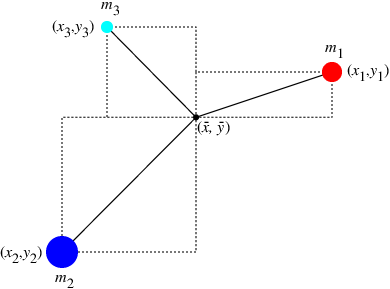
\includegraphics{11_4_COM_discrete}}
  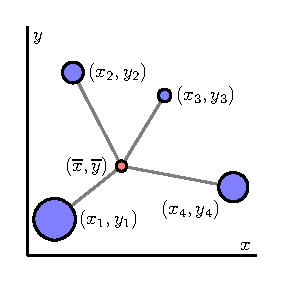
\includegraphics{figures/fig_11_4_masses.eps}
\end{center}
\caption{A center of mass $(\overline{x}, \overline{y})$ of four masses.}
\label{F:11.4.COM}
\end{figure}

Each mass exerts a force (called a \emph{moment}) around the lines $x=\overline{x}$ and $y=\overline{y}$ that causes the system to tilt in the direction of the mass. These moments are dependent on the mass and the distance from the given line. Let $(x_1,y_1)$ be the location of mass $m_1$, $(x_2,y_2)$ the location of mass $m_2$, etc. In order to balance perfectly, the moments in the $x$ direction and in the $y$ direction must be in equilibrium. We determine these moments and solve the resulting system to find the equilibrium point $(\overline{x}, \overline{y})$ at the center of mass.

The force that mass $m_1$ exerts to tilt the system from the line $y=\overline{y}$ is
\[m_1g(\overline{y} - y_1),\]
where $g$ is the gravitational constant. Similarly, the force mass $m_2$ exerts to tilt the system from the line $y= \overline{y}$ is
\[m_2g(\overline{y}-y_2).\]
In general, the force that mass $m_k$ exerts to tilt the system from the line $y= \overline{y}$ is
\[m_kg(\overline{y}-y_k).\]
For the system to balance, we need the forces to sum to 0, so that
\[\sum_{k=1}^N m_kg(\overline{y}-y_k) = 0.\]
Solving for $\overline{y}$, we find that
\[\overline{y} = \frac{\sum_{k=1}^N m_ky_k}{\sum_{k=1}^N m_k}.\]
A similar argument shows that
\[\overline{x} = \frac{\sum_{k=1}^N m_kx_k}{\sum_{k=1}^N m_k}.\]
The value $M_x~=~\sum_{k=1}^N m_ky_k$ is called the \emph{total moment} with respect to the $x$-axis; $M_y~=~\sum_{k=1}^N m_kx_k$ is the \emph{total moment} with respect to the $y$-axis.  Hence, the respective quotients of the moments to the total mass, $M$,  determines the center of mass of a point-mass system: $$(\overline{x}, \overline{y}) = \left(\frac{M_y}{M}, \frac{M_x}{M}\right).$$

Now, suppose that rather than a point-mass system, we have a continuous lamina with a variable mass-density $\delta(x, y)$. We may estimate its center of mass by partitioning the lamina into $mn$ subrectangles of equal area $\Delta A$, and treating the resulting partitioned lamina as a point-mass system.  In particular, we select a point $(x_{ij}^*,y_{ij}^*)$ in the $ij$th subrectangle, and observe that the quanity
\[\delta(x_{ij}^*,y_{ij}^*) \Delta A\]
is density times area, so $\delta(x_{ij}^*,y_{ij}^*) \Delta A$ approximates the mass of the small portion of the lamina determined by the subrectangle $R_{ij}$. 

We now treat $\delta(x_{ij}^*,y_{ij}^*) \Delta A$ as a point mass at the point $(x_{ij}^*,y_{ij}^*)$. The coordinates $(\overline{x}, \overline{y})$ of the center of mass of these $mn$ point masses are thus given by
\[\overline{x} = \frac{\sum_{j=1}^n \sum_{i=1}^m x_{ij}^*\delta(x_{ij}^*,y_{ij}^*) \Delta A}{\sum_{j=1}^n\sum_{i=1}^m \delta(x_{ij}^*,y_{ij}^*) \Delta A} \ \ \ \ \ \text{ and } \ \ \ \ \ \overline{y} = \frac{\sum_{j=1}^n \sum_{i=1}^m y_{ij}^*\delta(x_{ij}^*,y_{ij}^*) \Delta A}{\sum_{j=1}^n\sum_{i=1}^m \delta(x_{ij}^*,y_{ij}^*) \Delta A}.\]
If we take the limit as $m$ and $n$ go to infinity, we obtain the exact center of mass $(\overline{x}, \overline{y})$ of the continuous lamina.

\vspace*{5pt}
\nin \framebox{\hspace*{3 pt}
\parbox{6.25 in}{The coordinates $(\overline{x}, \overline{y})$ of the \textbf{center of mass of a lamina}\index{double integral!center of mass of a lamina} $D$ with density $\delta = \delta(x,y)$ are given by
\[\overline{x} = \frac{\iint_D x\delta(x,y) \, dA}{\iint_D \delta(x,y) \, dA} \ \ \ \ \ \text{ and } \ \ \ \ \ \overline{y} = \frac{\iint_D y\delta(x,y) \, dA}{\iint_D \delta(x,y) \, dA}.\]
} \hspace*{3 pt}}
\vspace*{5pt}

The numerators of $\overline{x}$ and $\overline{y}$ are called the respective \emph{moments}\index{moments about coordinate axes} of the lamina about the coordinate axes. Thus, the moment of a lamina $D$ with density $\delta = \delta(x,y)$ about the $y$-axis is
\[M_y = \iint_D x\delta(x,y) \, dA\]
and the moment of  $D$ about the $x$-axis is
\[M_x = \iint_D y\delta(x,y) \, dA.\]
If $M$ is the mass of the lamina, it follows that the center of mass is $(\overline{x}, \overline{y}) = \left(\frac{M_y}{M}, \frac{M_x}{M}\right)$. 
\begin{activity} \label{A:11.4.4} In this activity we determine integrals that represent the center of mass of a lamina $D$ described by the triangular region bounded by the $x$-axis and the lines $x = 1$ and $y = 2x$ in the first quadrant if the density at point $(x, y)$ is $\delta(x, y) = 6x + 6y + 6$. A picture of the lamina is shown in Figure \ref{F:11.4.COM_ex_1}.
\begin{figure}[ht]
\begin{center}
%\resizebox{!}{2.0in}{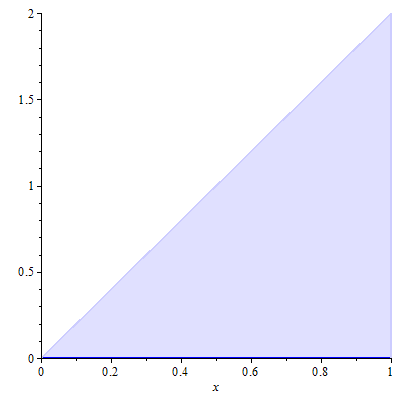
\includegraphics{11_4_COM_ex_1}}
  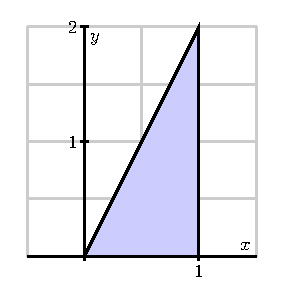
\includegraphics{figures/fig_11_4_triangle.eps}
\end{center}
\caption{The lamina bounded by the $x$-axis and the lines $x = 1$ and $y = 2x$ in the first quadrant.}
\label{F:11.4.COM_ex_1}
\end{figure}

    \ba
    \item Set up an iterated integral that represents the mass of the lamina.


    \item Assume the mass of the lamina is 14. Set up two iterated integrals that represent the coordinates of the center of mass of the lamina.


    \ea


\end{activity}
\begin{smallhint}

\end{smallhint}
\begin{bighint}

\end{bighint}
\begin{activitySolution}
\ba
\item The mass $M$ of the lamina is given by $\ds \int \int_D \delta(x,y) \, dA$. To calculate this mass, we set up an iterated integral, integrating first with respect to $y$ then $x$:
\[M = \int \int_D \delta(x,y) \, dA = \int_0^1 \int_0^{2x} (6x+6y+6) \, dy \, dx.\]
%\begin{align*}
%M &= \int \int_D \delta(x,y) \, dA \\	&= \int_0^1 \int_0^{2x} (6x+6y+6) \, dy \, dx \\
%	&= \int_0^1 \left[6xy+3y^2+6y\right]\biggm|_{0}^{2x} \, dx \\
%	&= \int_0^1 24x^2+12x \, dx \\
%	&= \left[8x^3+6x^2\right]\biggm|_0^1 \\
%	&= 14.
%\end{align*}

\item The $x$ coordinate of the center of mass is given by $\ds \frac{\int \int_D x \delta(x,y) \, dA}{14}$. An iterated integral that gives us this $x$ coordinate is 
\[\frac{1}{14}\int \int_D x \delta(x,y) \, dA = \frac{1}{14} \int_0^1 \int_0^{2x} x(6x+6y+6) \, dy \, dx.\]
%We need to evaluate the double integral
%$\ds \int \int_D x \delta(x,y) \, dA$ to complete this calculation:
%\begin{align*}
%\int \int_D x \delta(x,y) \, dA &= \int_0^1 \int_0^{2x} (6x^2+6xy+6x) \, dy \, dx \\
%	&= \int_0^1 \left[6x^2y+3xy^2+6xy\right]\biggm|_0^{2x} \, dx \\
%	&= \int_0^1 24x^3+12x^2 \, dx \\
%	&= \left[6x^4+4x^3\right]\biggm|_0^1 \\
%	&= 10.
%\end{align*}
%So the $x$ coordinate of the center of mass of the lamina is $\frac{10}{14} = \frac{5}{7}$.

The $y$ coordinate of the center of mass is given by $\ds \frac{\int \int_D y \delta(x,y) \, dA}{14}$. An iterated integral that gives us this $y$ coordinate is 
\[\frac{1}{14}\int \int_D y \delta(x,y) \, dA = \frac{1}{14} \int_0^1 \int_0^{2x} y(6x+6y+6) \, dy \, dx.\]
%We need to evaluate the double integral
%$\ds \int \int_D y \delta(x,y) \, dA$ to complete this calculation:
%\begin{align*}
%\int \int_D y \delta(x,y) \, dA &= \int_0^1 \int_0^{2x} (6xy+6y^2+6y) \, dy \, dx \\
%	&= \int_0^1 \left[3xy^2+2y^3+3y^2\right]\biggm|_0^{2x} \, dx \\
%	&= \int_0^1 28x^3+12x^2 \, dx \\
%	&= \left[7x^4+4x^3\right]\biggm|_0^1 \\
%	&= 11.
%\end{align*}
%So the $y$ coordinate of the center of mass of the lamina is $\frac{11}{14}$ and the center of mass of the lamina is $\left(\frac{5}{7}, \frac{11}{14}\right)$.
\ea

\end{activitySolution}
\aftera


%\begin{activity} \label{A:11.4.5} Let $D$ be a half-disk lamina of radius 3 in quadrants IV and I, centered at the origin as in Activity \ref{A:11.4.3}.  Assume the density at point $(x,y)$ is equal to $x$. Before doing any calculations, what do you expect the $y$-coordinate of the center of mass to be? Why? Now find the center of mass of the lamina. Use appropriate technology to evaluate the integrals. 

\end{activity}
\begin{smallhint}

\end{smallhint}
\begin{bighint}

\end{bighint}
\begin{activitySolution}
We calculated that mass of the lamina to be 18 in Activity \ref{A:11.4.3}. So the $x$-coordinate $\overline{x}$ of the center of mass of the lamina is given by 
\[\overline{x} = \frac{1}{18} \int_{-3}^{3} \int_{0}^{\sqrt{9-y^2}} x^2 \, dx \, dy.\]
Wolfram$|$Alpha gives this value as $\frac{9}{16} \pi$. 

Similarly, the $y$-coordinate $\overline{y}$ of the center of mass of the lamina is given by  
\[\overline{y} = \frac{1}{18} \int_{-3}^{3} \int_{0}^{\sqrt{9-y^2}} xy \, dx \, dy.\]
Wolfram$|$Alpha gives this value as $0$, which we should suspect due to the symmetry of the lamina around the $x$-axis.  
\end{activitySolution}
\aftera


\subsection*{Probability}

Calculating probabilities is a very important application of integration in the physical, social, and life sciences. To understand the basics, consider the game of darts in which a player throws a dart at a board and tries to hit a particular target. Let us suppose that a dart board is in the form of a disk $D$ with radius 10 inches. If we assume that a player throws a dart at random, and is not aiming at any particular point, then it is equally probable that the dart will strike any single point on the board. For instance, the probability that the dart will strike a particular 1 square inch region is $\frac{1}{100 \pi}$, or the ratio of the area of the desired target to the total area of $D$ (assuming that the dart thrower always hits the board itself at some point). Similarly, the probability that the dart strikes a point in the disk $D_3$ of radius 3 inches is given by the area of $D_3$ divided by the area of $D$. In other words, the probability that the dart strikes the disk $D_3$ is
\[\frac{9 \pi}{100\pi} = \iint_{D_3} \frac{1}{100 \pi} \, dA.\]
The integrand, $\frac{1}{100\pi}$, may be thought of as a \emph{distribution function}, describing how the dart strikes are distributed across the board. In this case the distribution function is constant since we are assuming a uniform distribution, but we can easily envision situations where the distribution function varies.  For example, if the player is fairly good and is aiming for the bulls eye (the center of $D$), then the distribution function $f$ could be skewed toward the center, say
\[f(x,y) = K e^{-(x^2+y^2)}\]
for some constant positive $K$. If we assume that the player is consistent enough so that the dart always strikes the board, then the probability that the dart strikes the board somewhere is 1, and the distribution function $f$ will have to satisfy\footnote{This makes $K = \frac{1}{\pi\left(1-e^{-100}\right)}$, which you can check.}
\[\iint_D f(x,y) \, dA = 1.\]
For such a function $f$, the probability that the dart strikes in the disk $D_1$ of radius 1 would be
\[\iint_{D_1} f(x,y) \, dA.\]
Indeed, the probability that the dart strikes in any region $R$ that lies within $D$ is given by
\[\iint_R f(x,y) \, dA.\]

The preceding discussion highlights the general idea behind calculating probabilities. We assume we have a \emph{joint probability density function}\index{joint probability density function} $f$, a function of two independent variables $x$ and $y$ defined on a domain $D$ that satisfies the conditions
\begin{itemize}
\item $f(x,y) \geq 0$ for all $x$ and $y$ in $D$,
\item the probability that $x$ is between some values $a$ and $b$ while $y$ is between some values $c$ and $d$ is given by
\[\int_a^b \int_c^d f(x,y) \, dy \, dx,\]
\item The probability\index{double integral!probability} that the point $(x,y)$ is in $D$ is 1, that is
\begin{equation} \label{eq:11.4.pdf}
\iint_D f(x,y) \, dA = 1.
\end{equation}
\end{itemize}
Note that it is possible that $D$ could be an infinite region and the limits on the integral in Equation~(\ref{eq:11.4.pdf}) could be infinite. When we have such a probability density function $f=f(x,y)$, the probability that the point $(x,y)$ is in some region $R$ contained in the domain $D$ (the notation we use here is ``$P((x,y)\in R)$'') is determined by
\[P((x,y)\in R) = \iint_R f(x,y) \, dA.\]

\begin{activity} \label{A:11.4.6} A firm manufactures smoke detectors. Two components for the detectors come from different suppliers -- one in Michigan and one in Ohio. The company studies these components for their reliability and their data suggests that if $x$ is the life span (in years) of a randomly chosen component from the Michigan supplier and $y$ the life span (in years) of a randomly chosen component from the Ohio supplier, then the joint probability density function $f$ might be given by
\[f(x,y) = e^{-x} e^{-y}.\]
    \ba
    \item Theoretically, the components might last forever, so the domain $D$ of the function $f$ is the set $D$ of all $(x,y)$ such that $x \ge 0$ and $y \ge 0$. To show that $f$ is a probability density function on $D$ we need to demonstrate that
        \[\int \int_D f(x,y) \, dA = 1,\]
        or that
        \[\int_0^{\infty} \int_0^{\infty} f(x,y) \, dy \, dx = 1.\]
        Use your knowledge of improper integrals to verify that $f$ is indeed a probability density function.

    \item Assume that the smoke detector fails only if both of the supplied components fail. To determine the probability that a randomly selected detector will fail within one year, we will need to determine the probability that the life span of each component is between 0 and 1 years. Set up an appropriate iterated integral, and evaluate the integral to determine the probability.
    
    \item What is the probability that a randomly chosen smoke detector will fail between years 3 and 7?
    
    \item Suppose that the manufacturer determines that one of the components is more likely to fail than the other, and hence conjectures that the probability density function is instead $f(x,y) = K e^{-x} e^{-2y}.$  What is the value of $K$?

    \ea

\end{activity}
\begin{smallhint}

\end{smallhint}
\begin{bighint}

\end{bighint}
\begin{activitySolution}
\ba
\item We evaluate the double integral to determine if $f$ is a probability density function:
\begin{align*}
\int_0^{\infty} \int_0^{\infty} f(x,y) \, dy \, dx &= \int_0^{\infty} \int_0^{\infty} e^{-x} e^{-y} \, dy \, dx \\
	&= \int_0^{\infty} e^{-x} \left( \int_0^{\infty}  e^{-y} \, dy \right) \, dx \\
	&= \int_0^{\infty} e^{-x} \left(\lim_{b \to \infty} \int_0^{b}  e^{-y} \, dy \right) \, dx \\
	&= \int_0^{\infty} e^{-x} \left(\lim_{b \to \infty} \left. -e^{-y} \right|_0^{b} \right) \, dx \\
	&= \int_0^{\infty} e^{-x} \left(\lim_{b \to \infty} -e^{-b}+1 \right) \, dx \\
	&= \int_0^{\infty} e^{-x} (1) \, dx \\
	&= \lim_{b \to \infty} \int_0^{b}  e^{-x} \, dx \\
	&= \lim_{b \to \infty} \left. -e^{-x} \right|_0^{b} \\
	&= \lim_{b \to \infty} -e^{-b}+1 \\
	&= 1.
\end{align*}
So $f$ is a probability density function.
	

\item We need both components to have a life span of 1 year or less, so the probability that a randomly selected detector will fail within one year is
\begin{align*}
\int_0^1 \int_0^1 f(x,y) \, dy \, dx &= \int_0^1 \int_0^1 e^{-x} e^{-y} \, dy \, dx \\
	&= \int_0^1  -e^{-x} e^{-y} \bigm|_{y=0}^1 \, dx \\
	&= \int_0^1  e^{-x} \left(1-\frac{1}{e}\right) \, dx \\
	&= \left(1-\frac{1}{e}\right) (-e^{-x})\bigm|_{x=0}^1 \\
	&= \left(1-\frac{1}{e}\right)^2.
\end{align*}
So the probability that a randomly selected detector will fail within one year is approximately 40\%.

\item We need both components to have a life span of between 3 and 7 years, so the probability that a randomly selected detector will fail within 3 to 7 years is
\begin{align*}
\int_3^7 \int_3^7 f(x,y) \, dy \, dx &= \int_3^7 \int_3^7 e^{-x} e^{-y} \, dy \, dx \\
	&= \int_3^7  -e^{-x} e^{-y} \bigm|_{y=3}^7 \, dx \\
	&= \int_3^7  e^{-x} \left(\frac{1}{e^3}-\frac{1}{e^7}\right) \, dx \\
	&= \left(\frac{1}{e^3}-\frac{1}{e^7}\right) (-e^{-x})\bigm|_{x=3}^7 \\
	&= \left(\frac{1}{e^3}-\frac{1}{e^7}\right)^2.
\end{align*}
This amounts to approximately 0.24\%. 

\item To find $K$ we need to determine when 
\[\int_0^{\infty} \int_0^{\infty} f(x,y) \, dy \, dx = 1.\]
We evaluate the iterated integral to determine the value of $K$:
\begin{align*}
\int_0^{\infty} \int_0^{\infty} f(x,y) \, dy \, dx &= \int_0^{\infty} \int_0^{\infty} Ke^{-x} e^{-2y} \, dy \, dx \\
	&= K\int_0^{\infty} e^{-x} \left( \int_0^{\infty}  e^{-2y} \, dy \right) \, dx \\
	&= K\int_0^{\infty} e^{-x} \left(\lim_{b \to \infty} \int_0^{b}  e^{-2y} \, dy \right) \, dx \\
	&= K\int_0^{\infty} e^{-x} \left(\lim_{b \to \infty} \left. -\frac{1}{2}e^{-2y} \right|_0^{b} \right) \, dx \\
	&= K\int_0^{\infty} e^{-x} \left(\lim_{b \to \infty} -\frac{1}{2}(e^{-2b}-1) \right) \, dx \\
	&= \frac{K}{2}\int_0^{\infty} e^{-x}  \, dx \\
	&= \frac{K}{2}\lim_{b \to \infty} \int_0^{b}  e^{-x} \, dx \\
	&= \frac{K}{2}\lim_{b \to \infty} \left. -e^{-x} \right|_0^{b} \\
	&= \frac{K}{2}\lim_{b \to \infty} -e^{-b}+1 \\
	&= \frac{K}{2}.
\end{align*}
So we need to have $K = 2$ for $f$ to be a probability density function.

\ea
\end{activitySolution}
\aftera




%\begin{activity} \label{A:11.4.7} Let $x$ denote the time (in minutes) that a person spends waiting in a checkout line at a grocery store and $y$ the time (in minutes) that it takes to check out. Set up a double integral that will determine the probability that you will spend no more than 10 minutes waiting and then checking out at this grocery store if the joint probability density function for $x$ and $y$ is
\[f(x,y) = \frac{1}{8} e^{-x/4-y/2}.\]

\end{activity}
\begin{smallhint}

\end{smallhint}
\begin{bighint}

\end{bighint}
\begin{activitySolution}
We need to have $x+y = 10$ with $x$ between 0 and $10$, so a double integral that represents the probability that you will spend no more than 10 minutes waiting and then checking out at this grocery store is
\[\int_0^{10} \int_0^{10-x} f(x,y) \, dy \, dx.\]
\end{activitySolution}
\aftera


\begin{summary}
\item The mass of a lamina $D$ with a mass density function $\delta = \delta(x,y)$ is  $\iint_D \delta(x,y) \, dA.$

\item The area of a region $D$ in the plane has the same numerical value as the volume of a solid of uniform height 1 and base $D$, so the area of $D$ is given by $\iint_D 1 \, dA.$   
    
\item The center of mass, $(\overline{x},\overline{y})$, of a continuous lamina with a variable density $\delta(x,y)$ is given by \[\overline{x} = \frac{\iint_D x\delta(x,y) \, dA}{\iint_D \delta(x,y) \, dA} \ \ \ \ \ \text{ and } \ \ \ \ \ \overline{y} = \frac{\iint_D y\delta(x,y) \, dA}{\iint_D \delta(x,y) \, dA}.\]

\item Given a joint probability density function $f$ is a function of two independent variables $x$ and $y$ defined on a domain $D$, 
if $R$ is some subregion of $D$, then the probability that $(x,y)$ is in $R$ is given by
\[\iint_R f(x,y) \, dA.\]
\end{summary}

\nin \hrulefill

\begin{exercises} 

\item A triangular plate is bounded by the graphs of the equations $y = 2x$, $y = 4x$, and $y = 4$.  The plate's density at $(x,y)$ is given by  $\delta(x,y) = 4xy^2 + 1$, measured in grams per square centimeter (and $x$ and $y$ are measured in centimeters).  
	
\ba
	\item Set up an iterated integral whose value is the mass of the plate. Include a labeled sketch of the region of integration.  Why did you choose the order of integration you did?  
	\item Determine the mass of the plate.    
	\item Determine the exact center of mass of the plate.  Draw and label the point you find on your sketch from (a).	
	\item  What is the average density of the plate?  Include units on your answer.
\ea

\begin{exerciseSolution}
\ba
	\item We obtain mass by integrating density, so the mass of the plate is
\[\int_{y=0}^{y=4} \int_{x=y/4}^{x=y/2} 4xy^2 + 1 \, dx \, dy.\]
If we instead integrate first with respect to $y$, the fact that the curve on the bottom will change over the interval means that will would need two iterated integrals instead of just one.   
	\item To find the mass $m$ we evaluate the iterated integral:
\begin{align*}
m&=\int_{y=0}^{y=4} \int_{x=y/4}^{x=y/2} 4xy^2 + 1 \, dx \, dy \\
	&= \int_{y=0}^{y=4} \left(2x^2y^2+x\right)\biggm|_{x=y/4}^{x=y/2} \, dy \\
	&= \int_{y=0}^{y=4} \left[\left(\frac{y^4}{2} + \frac{y}{2} \right) - \left(\frac{y^4}{8}+\frac{y}{4} \right)  \right] \, dy \\
	&= \int_{y=0}^{y=4} \left[\frac{3y^4}{8}+\frac{y}{4} \right] \, dy \\
	&= \left[\frac{3}{40}y^5 + \frac{y^2}{8} \right]  \int_{y=0}^{y=4}   \\
	&= \frac{3}{40}4^5 + \frac{4^2}{8}     \\
	&= \frac{394}{5}.
\end{align*}

	\item The center of mass of the plate is $(\overline{x}, \overline{y})$, where
\begin{align*}
\overline{x} &= \frac{1}{m} \int_{y=0}^{y=4} \int_{x=y/4}^{x=y/2} x(4xy^2 + 1) \, dx \, dy \\
	&= \frac{5}{394} \int_{y=0}^{y=4} \left(\frac{4}{3}x^3y^2+\frac{1}{2}x^2\right)\biggm|_{x=y/4}^{x=y/2} \, dy \\
	&= \frac{5}{394} \int_{y=0}^{y=4} \left[\left(\frac{1}{3}\frac{y^5}{2} + \frac{y^2}{8} \right) - \left(\frac{1}{3}\frac{y^5}{16}+\frac{y^2}{32} \right)  \right] \, dy \\
	&= \frac{5}{394} \int_{y=0}^{y=4} \left[\frac{7y^5}{48}+\frac{3y^2}{32} \right] \, dy \\
	&= \frac{5}{394} \left[\frac{7}{288}y^6 + \frac{y^3}{32} \right]  \int_{y=0}^{y=4}   \\
	&= \frac{5}{394} \left[\frac{7}{288}4^6 + \frac{4^3}{32}\right]     \\
	&= \frac{2285}{1773} \\
	&\approx 1.289.
\end{align*}
and
\begin{align*}
\overline{y} &= \frac{1}{m} \int_{y=0}^{y=4} \int_{x=y/4}^{x=y/2} y(4xy^2 + 1) \, dx \, dy \\
	&= \frac{5}{394} \int_{y=0}^{y=4} \left(2x^2y^3+xy\right)\biggm|_{x=y/4}^{x=y/2} \, dy \\
	&= \frac{5}{394} \int_{y=0}^{y=4} \left[\left(\frac{1}{2}y^5 + \frac{1}{2}y^2\right) - \left(\frac{1}{8}y^5+\frac{1}{4}y^2 \right)  \right] \, dy \\
	&= \frac{5}{394} \int_{y=0}^{y=4} \left[\frac{3}{8}y^5+\frac{1}{4}y^2 \right] \, dy \\
	&= \frac{5}{394} \left[\frac{1}{16}y^6 + \frac{1}{12}y^3 \right]  \int_{y=0}^{y=4}   \\
	&= \frac{5}{394} \left[\frac{1}{16}4^6 + \frac{1}{12}4^3 \right]     \\
	&= \frac{1960}{591} \\
	&\approx 3.316.
\end{align*}


	\item First note that the area $A$ of the plate is 
\begin{align*}
A &= \int_{y=0}^{y=4} \int_{x=y/4}^{x=y/2} 1 \, dx \, dy \\
	&= \int_{y=0}^{y=4} x\biggm|_{x=y/4}^{x=y/2}  \, dy \\
	&= \int_{y=0}^{y=4} \frac{y}{4}  \, dy \\
	&= \frac{y^2}{8}\biggm|_{y=0}^{y=4} \\
	&= 2.
\end{align*}
The average density of the plate is then 
\[\frac{1}{A} \int_{y=0}^{y=4} \int_{x=y/4}^{x=y/2} 4xy^2 + 1 \, dx \, dy = \frac{197}{5} \ \frac{\text{g}}{\text{cm}^2}.\]

\ea
\end{exerciseSolution}

\item Let $D$ be a half-disk lamina of radius 3 in quadrants IV and I, centered at the origin as in Activity \ref{A:11.4.3}.  Assume the density at point $(x,y)$ is equal to $x$. 
	\ba 
	    \item Before doing any calculations, what do you expect the $y$-coordinate of the center of mass to be? Why? 
	    \item Set up iterated integral expressions which, if evaluated, will determine the exact center of mass of the lamina. 
	    \item Use appropriate technology to evaluate the integrals to find the center of mass numerically.
	 \ea 
\begin{exerciseSolution}
	\ba
	\item Due to the symmetry of the lamina around the $x$-axis we should expect the $y$-coordinate of the center of mass to be 0. 

	\item We calculated that mass of the lamina to be 18 in Activity \ref{A:11.4.3}. So the $x$-coordinate $\overline{x}$ of the center of mass of the lamina is given by 
\[\overline{x} = \frac{1}{18} \int_{-3}^{3} \int_{0}^{\sqrt{9-y^2}} x^2 \, dx \, dy.\]
Similarly, the $y$-coordinate $\overline{y}$ of the center of mass of the lamina is given by  
\[\overline{y} = \frac{1}{18} \int_{-3}^{3} \int_{0}^{\sqrt{9-y^2}} xy \, dx \, dy.\]

	\item Wolfram$|$Alpha gives $\overline{x} = \frac{9}{16} \pi$ and $\overline{y} = 0$, as expected.   
	\ea
\end{exerciseSolution}

\item Let $x$ denote the time (in minutes) that a person spends waiting in a checkout line at a grocery store and $y$ the time (in minutes) that it takes to check out.  Suppose the joint probability density for $x$ and $y$ is
\[f(x,y) = \frac{1}{8} e^{-x/4-y/2}.\]

	\ba
		\item What is the exact probability that a person spends between 0 to 5 minutes waiting in line, and then 0 to 5 minutes waiting to check out?
		\item Set up, but do not evaluate, an iterated integral whose value determines the exact probability that a person spends at most 10 minutes total both waiting in line and checking out at this grocery store.
		\item Set up, but do not evaluate, an iterated integral expression whose value determines the exact probability that a person spends at least 10 minutes total both waiting in line and checking out, but not more than 20 minutes.
	\ea

\begin{exerciseSolution}
	\ba
	\item We want to have $0 \leq x \leq 5$ and $0 \leq y \leq 5$. So the probability that a person spends between 0 to 5 minutes waiting in line, and then 0 to 5 minutes waiting to check out is
	\begin{align*}
	\int_0^{5} \int_0^{5} f(x,y) \, dy \, dx &= \int_0^{5} \int_0^{5} \frac{1}{8} e^{-x/4-y/2} \, dy \, dx \\
		&= \int_0^{5} -\frac{1}{4} e^{-x/4-y/2}\biggm|_0^{5}  \, dx \\
		&= \int_0^{5} -\frac{1}{4} \left(e^{-x/4-5/2} - e^{-x/4}\right)  \, dx \\
		&= \left(e^{-x/4-5/2} - e^{-x/4}\right)\biggm|_{0}^{5} \\
		&= \left(e^{-15/4} - e^{-5/4}\right) - \left(e^{-5/2} - 1\right) \\
		&\approx 0.655.
	\end{align*}
So the probability is approximately 65.5\%. 

	\item We need to have $x+y = 10$ with $x$ between 0 and $10$, so an iterated integral that represents the probability that a person spends no more than 10 minutes waiting and then checking out at this grocery store is
\[\int_0^{10} \int_0^{10-x} f(x,y) \, dy \, dx.\]

	\item We need to have $10 \leq x+y \leq 20$ with $x$ between 0 and $20$, so an iterated integral that represents the probability that a person spends at least 10 minutes total both waiting in line and checking out, but not more than 20 minutes is 
\[\int_{10}^{20} \int_{10-x}^{20-x} f(x,y) \, dy \, dx.\]

	\ea
\end{exerciseSolution}

\end{exercises}

\afterexercises


\clearpage
